\subsection{Glyph: \glyph{Tag}}
\label{sec:tag}

A \glyph{tag} is a named handle, or reference, to another \glyph{BA} (\sect{af:biologicalActivity}) or \glyph{compartment} (\sect{compartment}) of the map. Together with the \glyph{submap terminal} (\sect{submapTerminal}), it allows linking glyphs of a map to their counterpart in a submap.

\begin{glyphDescription}

\glyphSboTerm Not applicable.

\glyphIncoming
One \glyph{equivalence arc} (\sect{equivalenceArc}).

\glyphOutgoing
None.

\glyphContainer A \glyph{tag} is represented by a rectangular shape fused to an empty arrowhead, as shown in \fig{tag}.
The incoming \glyph{equivalence arc} (\sect{equivalenceArc}) must be linked to the extremity of the arrowhead.

\glyphLabel A \glyph{tag} is identified by a label that is  a string of characters that may be distributed on several lines to improve readability.
The centre of the label must be placed on the centre of the shape.
The label may extend outside of the shape.

\glyphAux 
None.

\end{glyphDescription}

\begin{figure}[H]
  \centering
  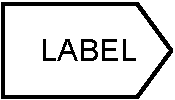
\includegraphics{images/build/tag.pdf}
  \caption{The \AF glyph for \glyph{tag}.}
  \label{fig:tag}
\end{figure}
